\chapter{Validating to BANFF}
\label{chap:banff_valid}
As outlined in \autoref{sec:oscchain}, T2K has two near-detector fitters: one Markov Chain Monte Carlo fitter (``MaCh3'') and one frequentist gradient descent fitter (``BANFF''). The results of the 2017 fits has been presented using the former, and this section shows the validation tests throughout the fitting process between the two fitters.

The validation procedure is not expected to entirely agree at all stages due to numerous technical and statistical differences. As covered earlier, a gradient descent minimiser is designed to find a global minimum of the test-statistic whereas a MCMC samples to build up a posterior distribution in high dimension. Comparing parameter values between the two is not a trivial exercise, and differences are expected. 

An example of a technical difference is MaCh3 evaluates the weights from cross-section parameter variations on GPGPUs\footnote{General Purpose Graphics Processing Units}, which involves floating point operations in 32 (float) rather than 64 bits (double). The effect of this on 35,000 events from run 3c is shown in \autoref{fig:cpu_vs_gpu_weight}, where we observe weight differences on the 1E-7 scale per event, which agrees well with the float vs double precision. Hence we expect small differences in event rates, although too small to notice in a likelihood evaluation.

\begin{figure}[h]
	\begin{subfigure}[t]{0.45\textwidth}
		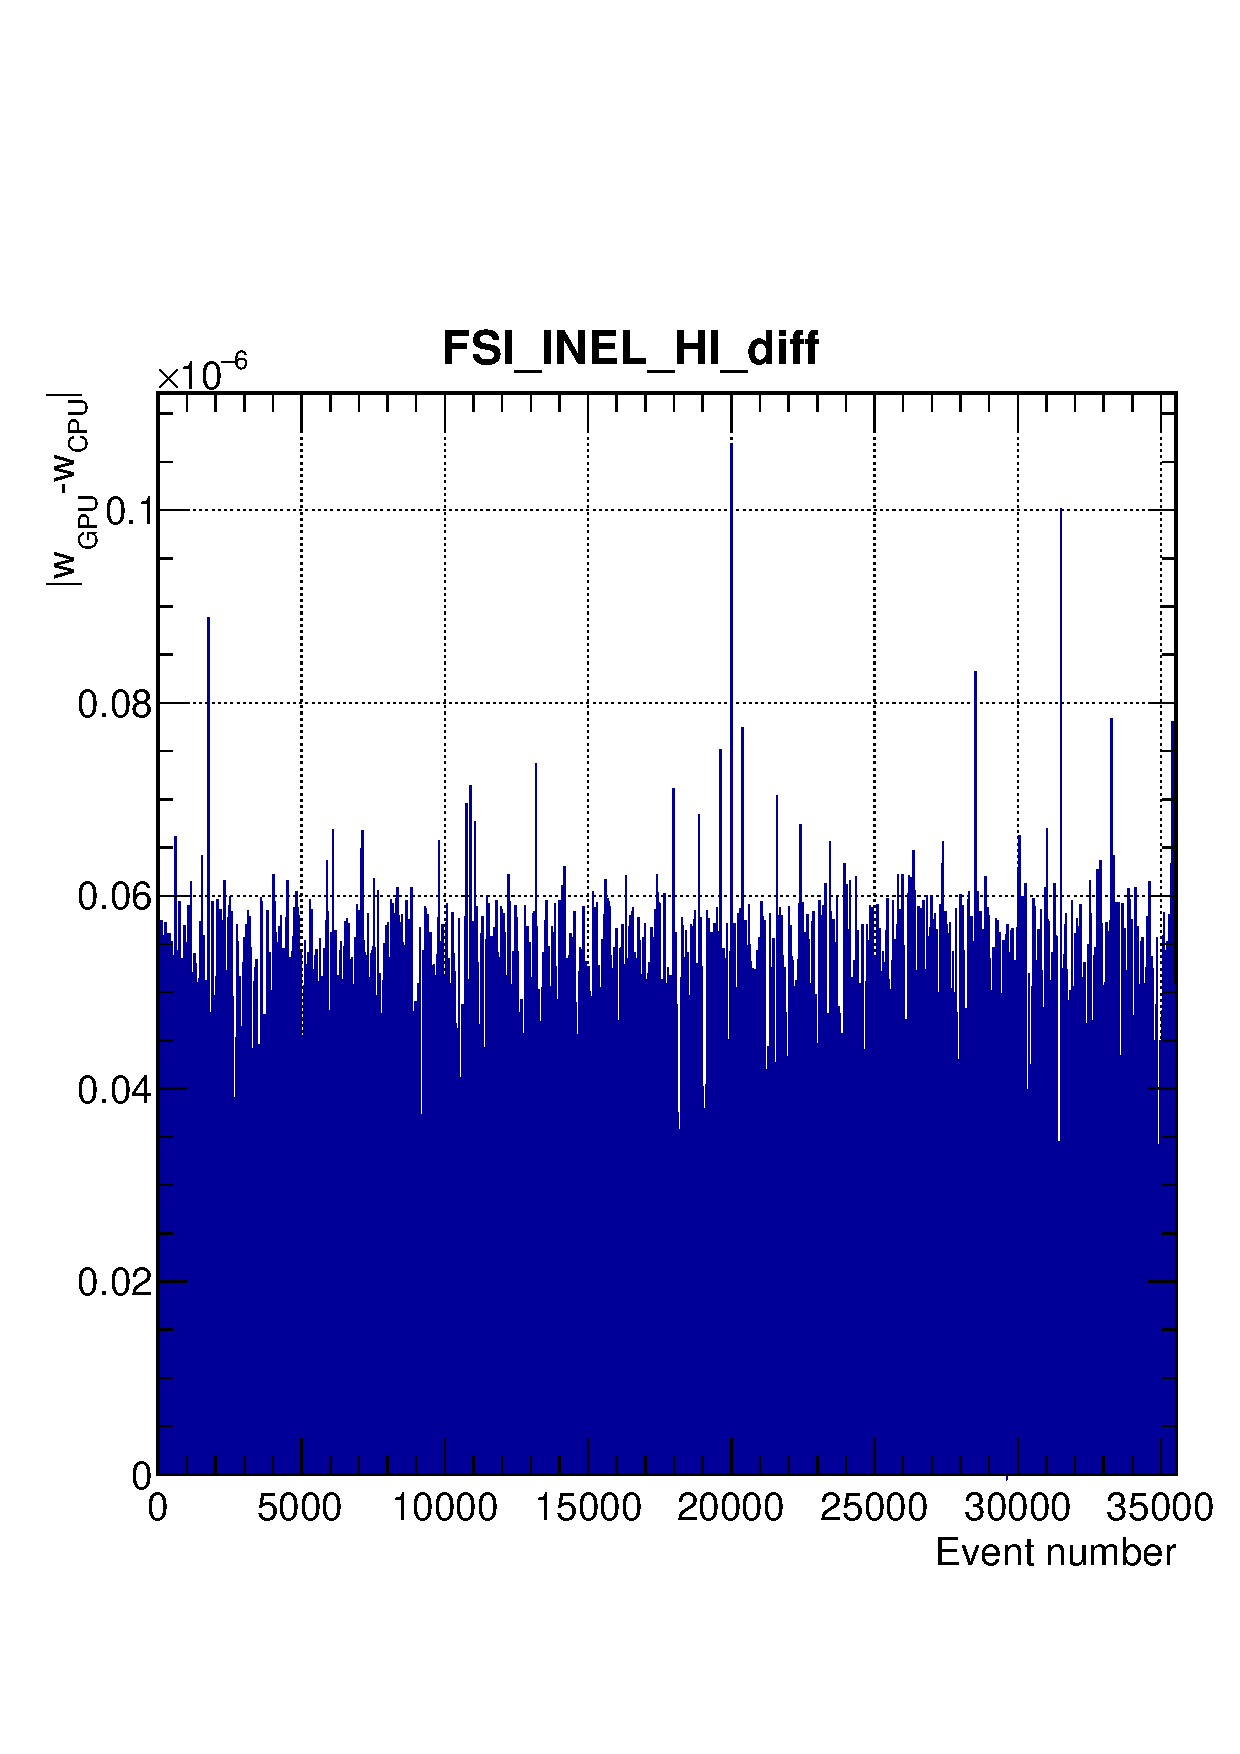
\includegraphics[width=\textwidth, trim={0mm 20mm 0mm 0mm}, clip, page=1]{figures/mach3/Asimov/fsi_inel_hi_diff}
	\end{subfigure}
	\begin{subfigure}[t]{0.45\textwidth}
		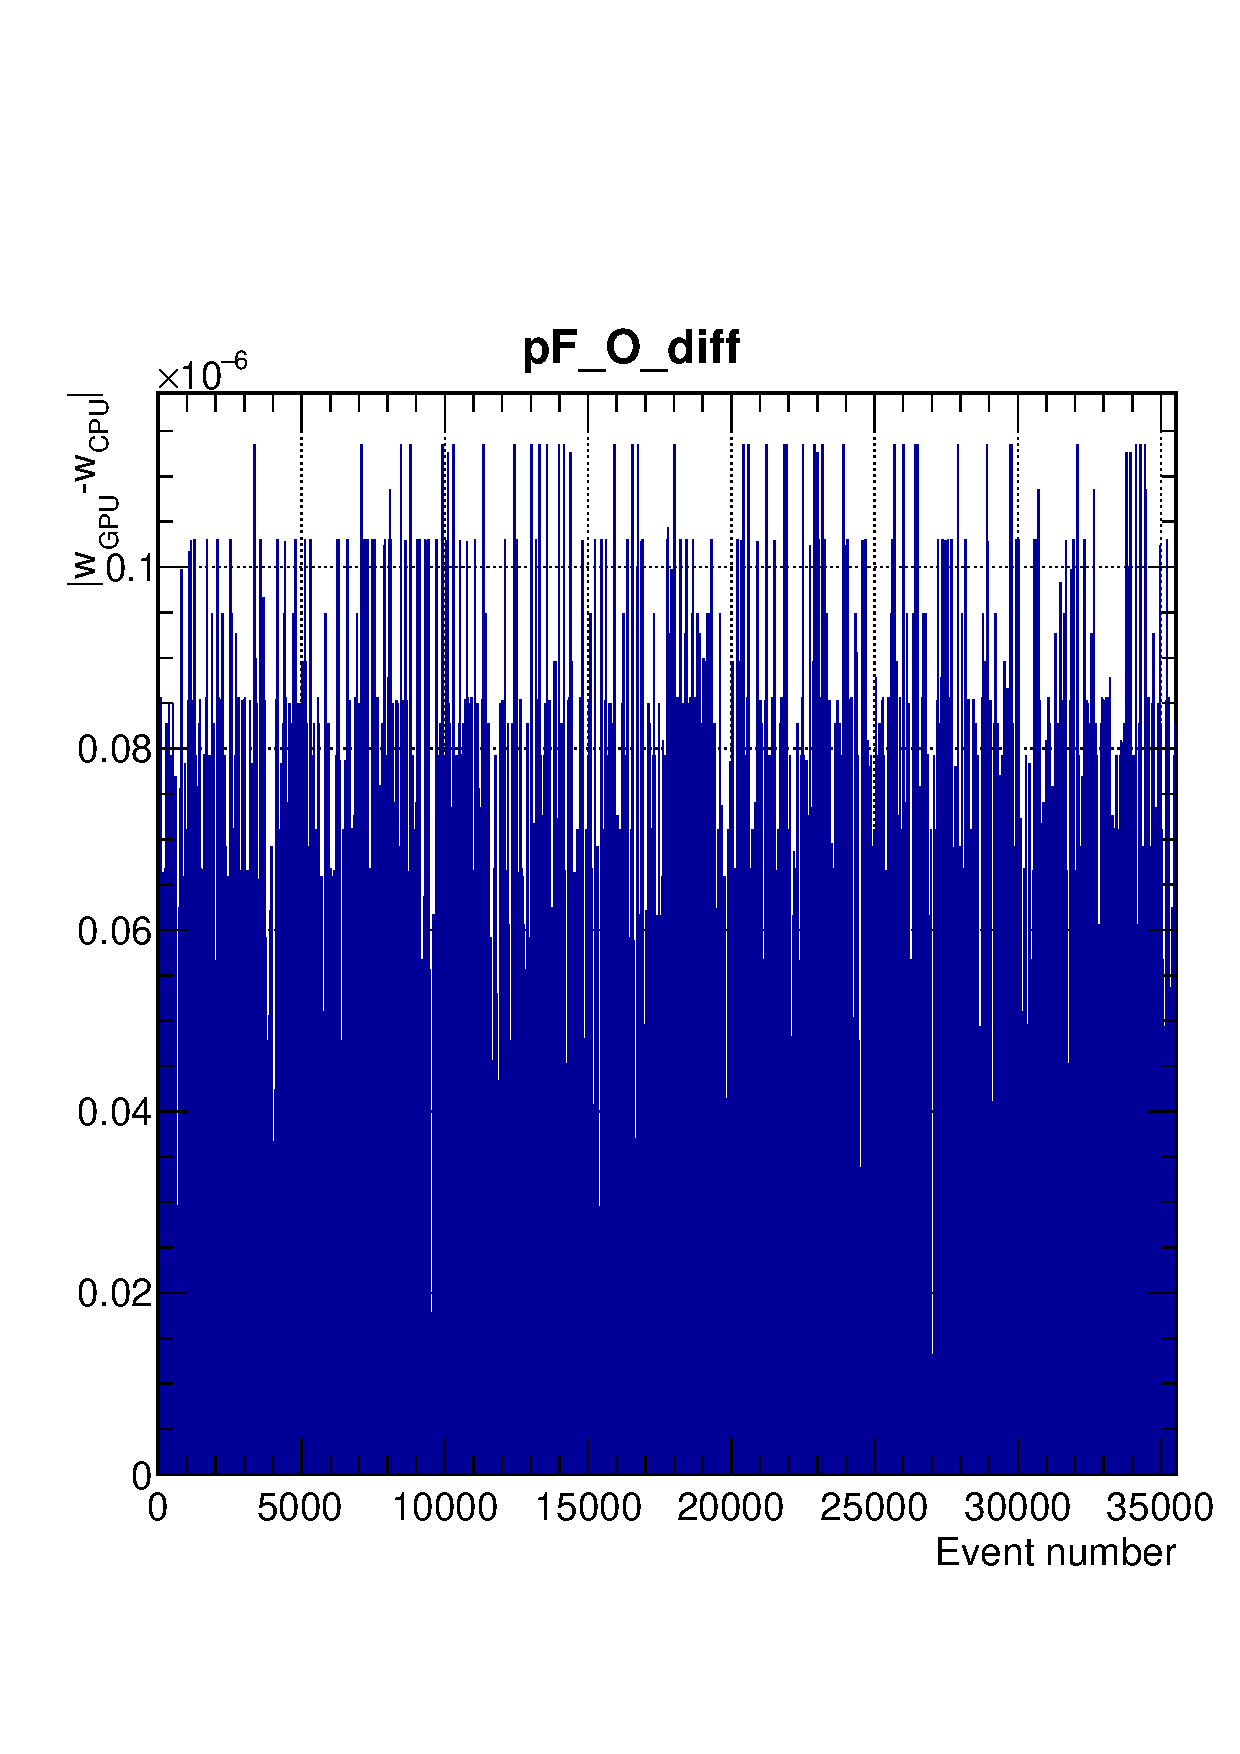
\includegraphics[width=\textwidth, trim={0mm 20mm 0mm 0mm}, clip, page=1]{figures/mach3/Asimov/pfo_diff}
	\end{subfigure}
	\caption{Absolute weight differences using a GPU versus CPU for a random parameter variation in MaCh3 for Run 3c Monte-Carlo}
	\label{fig:cpu_vs_gpu_weight}
\end{figure}

Weights from cross-section parameters were also compared for a selected few events and was found to be accurate to 1E-6. 

\section{Nominal model}
The nominal model and selection are run through both the MaCh3 and BANFF frameworks and the nominal event rates are compared in \autoref{tab:eventrate_banff_mach3}. The largest difference is seen in the FGD1 1Trk selection $\mathcal{O}(10^{-3})$ percent and the total difference is $\mathcal{O}(10^{-4})$ percent, which were deemed acceptable.
\begin{table}[h]
	\centering
	\begin{tabular}{ l | c c c c }
		\hline 
		\hline 
		Sample & Data  & BANFF & MaCh3 & $\frac{\text{BANFF-MaCh3}}{\text{BANFF}}$ \\ 
		\hline
		FGD1 0$\pi$ &  17136 &  16723.69 & 16723.8 & -6.60E-6 \\
		FGD1 1$\pi$ &  3954 &  4381.48 & 4381.47 & 2.28E-6\\ 
		FGD1 Other &  4149 &  3943.95 & 3943.95 & 0E0\\ 
		\hline
		FGD2 0$\pi$ &  17443 &  16959.19 & 16959.3 & -6.49E-6 \\
		FGD2 1$\pi$ &  3366 &  3564.23 & 3564.23 & 0E0\\
		FGD2 Other &  4075 &  3570.95 & 3570.94 & 2.80E-6 \\
		\hline
		FGD1 1Trk &  3527 &  3587.65 & 3587.77 & -3.34E-5\\ 
		FGD1 NTrk &  1054 &  1066.91 & 1066.91 & 0E0\\
		\hline
		FGD2 1Trk &  3732 &  3618.27 & 3618.29 & -5.53E-6 \\
		FGD2 NTrk &  1026 &  1077.24 & 1077.24 & 0E0 \\
		\hline
		FGD1 \numu 1Trk &  1363 &  1272.17 & 1272.17 & 0E0\\
		FGD1 \numu NTrk &  1370 &  1357.45 & 1357.45 & 0E0 \\
		\hline
		FGD2 \numu 1Trk &  1320 &  1262.63 & 1262.63 & 0E0 \\
		FGD2 \numu NTrk &  1253 &  1246.71 & 1246.71 & 0E0 \\
		\hline
		Total &  64768 &  63632.53 & 63632.9 & -5.81E-6 \\
		\hline
		\hline
	\end{tabular}
	\caption{BANFF and MaCh3 comparison of final event rates for the nominal model and data}
	\label{tab:eventrate_banff_mach3}
\end{table}

\autoref{fig:mach3_banff_prefit_fgd1} and \autoref{fig:mach3_banff_prefit_fgd2} show the 2D \pmu \cosmu distributions for FGD1 and FGD2 respectively, with BANFF-MaCh3 on the z-axis. We see the differences in \autoref{tab:eventrate_banff_mach3} come primarily from one or two bins, and it was found these differences were due to the interaction parameter evaluations mentioned earlier.
\begin{figure}[h]
	\begin{subfigure}[t]{0.32\textwidth}
		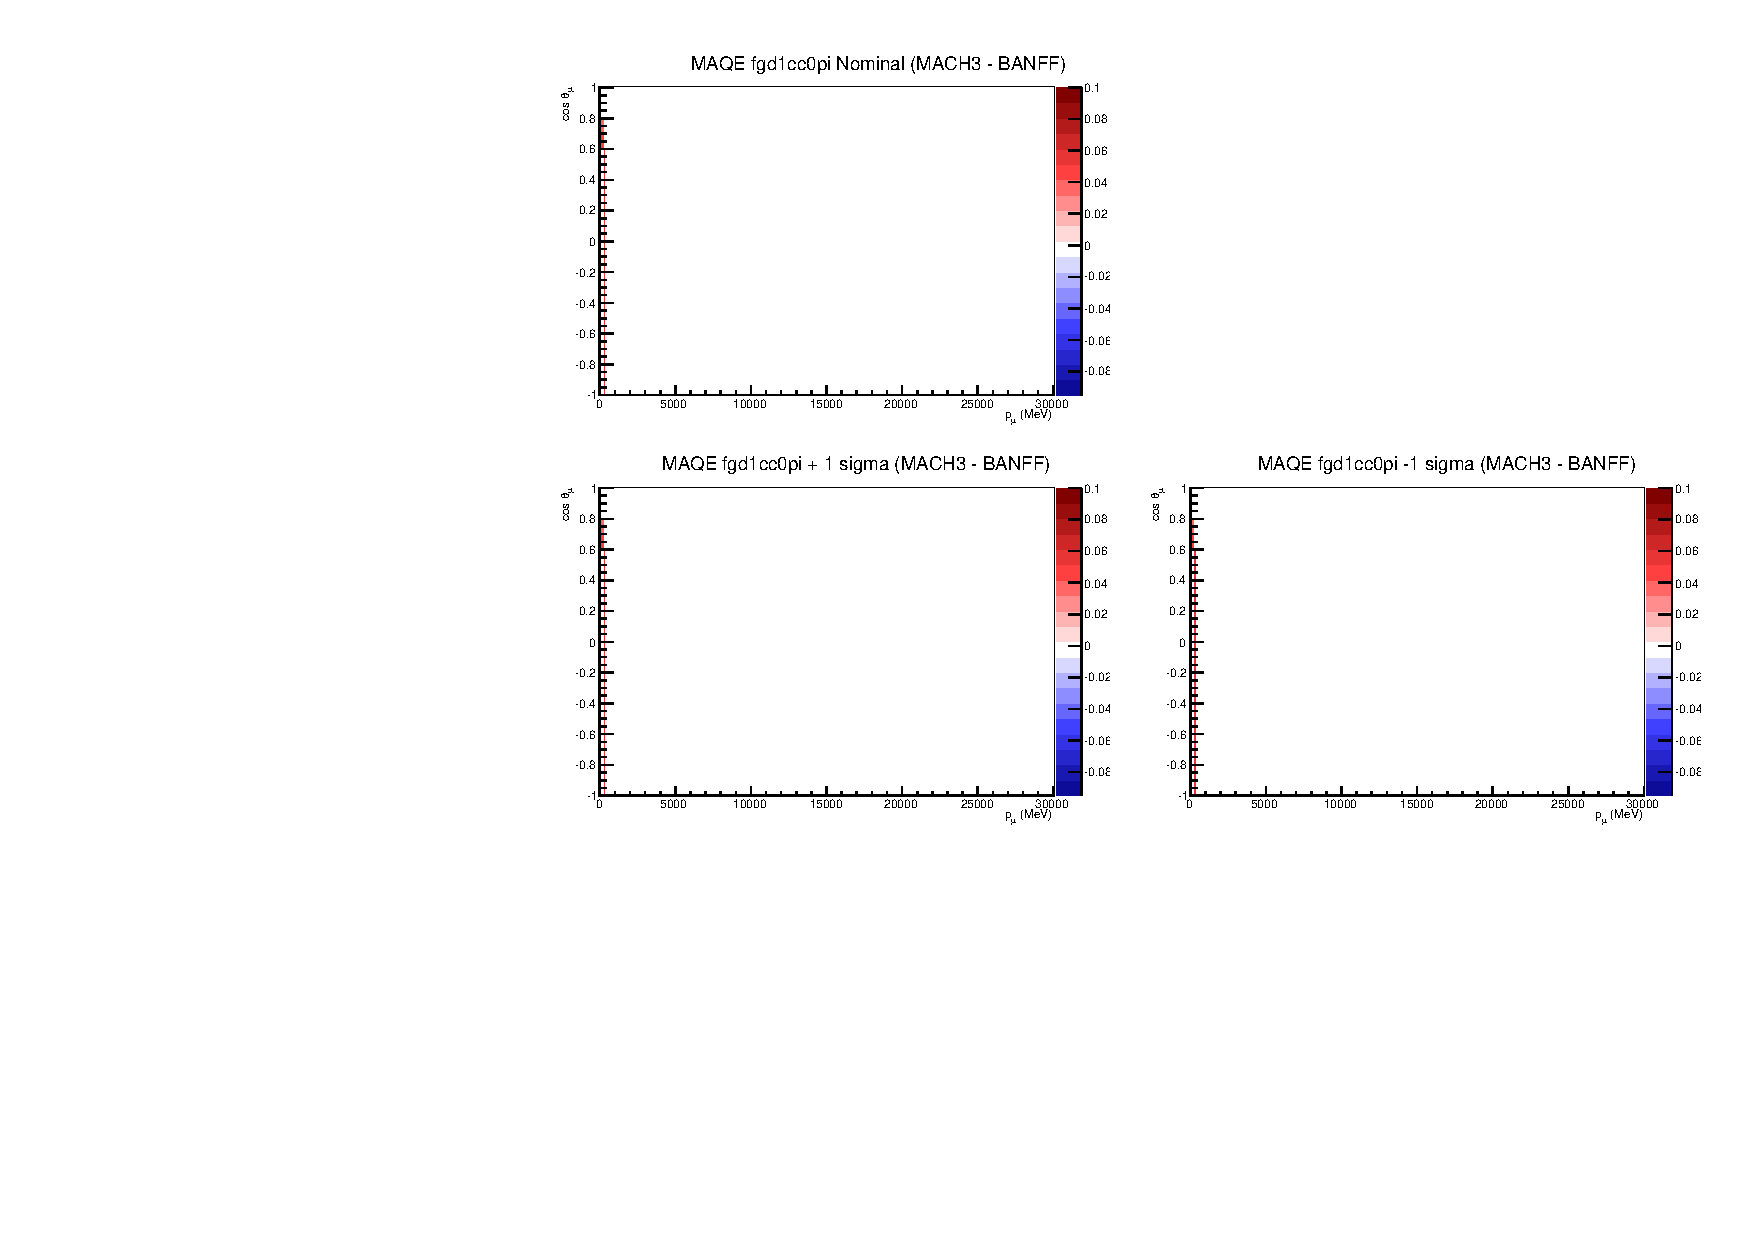
\includegraphics[width=\textwidth, trim={5mm 70mm 100mm 7mm}, clip, page=1]{figures/mach3/banff/momentumProjections_170328_withMACH3_MAQEonly}
		\caption{0$\pi$}
	\end{subfigure}
	\begin{subfigure}[t]{0.32\textwidth}
		\includegraphics[width=\textwidth, trim={5mm 70mm 100mm 7mm}, clip, page=2]{figures/mach3/banff/momentumProjections_170328_withMACH3_MAQEonly}
		\caption{1$\pi$}
	\end{subfigure}
	\begin{subfigure}[t]{0.32\textwidth}
		\includegraphics[width=\textwidth, trim={5mm 70mm 100mm 7mm}, clip, page=3]{figures/mach3/banff/momentumProjections_170328_withMACH3_MAQEonly}
		\caption{Other}
	\end{subfigure}
	
	\begin{subfigure}[t]{0.24\textwidth}
		\includegraphics[width=\textwidth, trim={5mm 70mm 100mm 7mm}, clip, page=4]{figures/mach3/banff/momentumProjections_170328_withMACH3_MAQEonly}
		\caption{1Trk}
	\end{subfigure}
	\begin{subfigure}[t]{0.24\textwidth}
		\includegraphics[width=\textwidth, trim={5mm 70mm 100mm 7mm}, clip, page=5]{figures/mach3/banff/momentumProjections_170328_withMACH3_MAQEonly}
		\caption{NTrk}
	\end{subfigure}
	\begin{subfigure}[t]{0.24\textwidth}
		\includegraphics[width=\textwidth, trim={5mm 70mm 100mm 7mm}, clip, page=6]{figures/mach3/banff/momentumProjections_170328_withMACH3_MAQEonly}
		\caption{\numu 1Trk}
	\end{subfigure}
	\begin{subfigure}[t]{0.24\textwidth}
		\includegraphics[width=\textwidth, trim={5mm 70mm 100mm 7mm}, clip, page=7]{figures/mach3/banff/momentumProjections_170328_withMACH3_MAQEonly}
		\caption{\numu NTrk}
	\end{subfigure}
	\caption{FGD1 selections showing the nominal MaCh3-BANFF events}
	\label{fig:mach3_banff_prefit_fgd1}
\end{figure}

\begin{figure}[h]
	\begin{subfigure}[t]{0.32\textwidth}
		\includegraphics[width=\textwidth, trim={5mm 70mm 100mm 7mm}, clip, page=8]{figures/mach3/banff/momentumProjections_170328_withMACH3_MAQEonly}
		\caption{0$\pi$}
	\end{subfigure}
	\begin{subfigure}[t]{0.32\textwidth}
		\includegraphics[width=\textwidth, trim={5mm 70mm 100mm 7mm}, clip, page=9]{figures/mach3/banff/momentumProjections_170328_withMACH3_MAQEonly}
		\caption{1$\pi$}
	\end{subfigure}
	\begin{subfigure}[t]{0.32\textwidth}
		\includegraphics[width=\textwidth, trim={5mm 70mm 100mm 7mm}, clip, page=10]{figures/mach3/banff/momentumProjections_170328_withMACH3_MAQEonly}
		\caption{Other}
	\end{subfigure}
	
	\begin{subfigure}[t]{0.24\textwidth}
		\includegraphics[width=\textwidth, trim={5mm 70mm 100mm 7mm}, clip, page=11]{figures/mach3/banff/momentumProjections_170328_withMACH3_MAQEonly}
		\caption{1Trk}
	\end{subfigure}
	\begin{subfigure}[t]{0.24\textwidth}
		\includegraphics[width=\textwidth, trim={5mm 70mm 100mm 7mm}, clip, page=12]{figures/mach3/banff/momentumProjections_170328_withMACH3_MAQEonly}
		\caption{NTrk}
	\end{subfigure}
	\begin{subfigure}[t]{0.24\textwidth}
		\includegraphics[width=\textwidth, trim={5mm 70mm 100mm 7mm}, clip, page=13]{figures/mach3/banff/momentumProjections_170328_withMACH3_MAQEonly}
		\caption{\numu 1Trk}
	\end{subfigure}
	\begin{subfigure}[t]{0.24\textwidth}
		\includegraphics[width=\textwidth, trim={5mm 70mm 100mm 7mm}, clip, page=14]{figures/mach3/banff/momentumProjections_170328_withMACH3_MAQEonly}
		\caption{\numu NTrk}
	\end{subfigure}
	\caption{FGD2 selections showing the nominal MaCh3-BANFF events}
	\label{fig:mach3_banff_prefit_fgd2}
\end{figure}

\section{Likelihood scans}
The likelihood scans in \autoref{sec:llh_scan} are also validated across the two groups. As then, likelihood response is scanned across a parameter one at a time, and all other parameters are fixed to their nominal values. This validation has two main purposes: checking the likelihood response of the prior term and the sample term. The plots shown below are for the total likelihood.

A selection of ND280 flux parameters are shown in \autoref{fig:banff_asimov_scan_ND280_flux}. We see very good agreement for the different groups of parameters, and all other flux parameters display this property.
\begin{figure}[h]
	\begin{subfigure}[t]{0.24\textwidth}
		\includegraphics[width=\textwidth, trim={0mm 0mm 0mm 11mm}, clip, page=4]{figures/mach3/banff/Asimov_scan_20July_flux_Full_LLHscan_18July_BeRPA_U_ND280logL_scan}
		\caption{FHC \numu 0.6-0.7 GeV}
	\end{subfigure}
	\begin{subfigure}[t]{0.24\textwidth}
		\includegraphics[width=\textwidth, trim={0mm 0mm 0mm 11mm}, clip, page=19]{figures/mach3/banff/Asimov_scan_20July_flux_Full_LLHscan_18July_BeRPA_U_ND280logL_scan}
		\caption{FHC \nue 0.7-0.8 GeV}
	\end{subfigure}
	\begin{subfigure}[t]{0.24\textwidth}
		\includegraphics[width=\textwidth, trim={0mm 0mm 0mm 11mm}, clip,page=36]{figures/mach3/banff/Asimov_scan_20July_flux_Full_LLHscan_18July_BeRPA_U_ND280logL_scan}
		\caption{RHC \numu 1.0-1.5 GeV}
	\end{subfigure}
	\begin{subfigure}[t]{0.24\textwidth}
		\includegraphics[width=\textwidth, trim={0mm 0mm 0mm 11mm}, clip,page=47]{figures/mach3/banff/Asimov_scan_20July_flux_Full_LLHscan_18July_BeRPA_U_ND280logL_scan}
		\caption{RHC \numu 0.8-1.5 GeV}
	\end{subfigure}
	\caption{Likelihood scan comparison between BANFF and MaCh3 for ND280 flux parameters}
	\label{fig:banff_asimov_scan_ND280_flux}
\end{figure}

\autoref{fig:banff_asimov_scan_SK_flux} shows the same parameters as in \autoref{fig:banff_asimov_scan_ND280_flux} but for SK. We again note perfect agreement for all parameters.
\begin{figure}[h]
	\begin{subfigure}[t]{0.24\textwidth}
		\includegraphics[width=\textwidth, trim={0mm 0mm 0mm 11mm}, clip, page=54]{figures/mach3/banff/Asimov_scan_20July_flux_Full_LLHscan_18July_BeRPA_U_ND280logL_scan}
		\caption{FHC \numu 0.6-0.7 GeV}
	\end{subfigure}
	\begin{subfigure}[t]{0.24\textwidth}
		\includegraphics[width=\textwidth, trim={0mm 0mm 0mm 11mm}, clip, page=69]{figures/mach3/banff/Asimov_scan_20July_flux_Full_LLHscan_18July_BeRPA_U_ND280logL_scan}
		\caption{FHC \nue 0.7-0.8 GeV}
	\end{subfigure}
	\begin{subfigure}[t]{0.24\textwidth}
		\includegraphics[width=\textwidth, trim={0mm 0mm 0mm 11mm}, clip,page=86]{figures/mach3/banff/Asimov_scan_20July_flux_Full_LLHscan_18July_BeRPA_U_ND280logL_scan}
		\caption{RHC \numu 1.0-1.5 GeV}
	\end{subfigure}
	\begin{subfigure}[t]{0.24\textwidth}
		\includegraphics[width=\textwidth, trim={0mm 0mm 0mm 11mm}, clip,page=97]{figures/mach3/banff/Asimov_scan_20July_flux_Full_LLHscan_18July_BeRPA_U_ND280logL_scan}
		\caption{RHC \numu 0.8-1.5 GeV}
	\end{subfigure}
	\caption{Likelihood scan comparison between BANFF and MaCh3 for SK flux parameters}
	\label{fig:banff_asimov_scan_SK_flux}
\end{figure}

\autoref{fig:banff_asimov_scan_xsec} shows the likelihood responses for a selection of interaction parameters, which also agree well.
\begin{figure}[h]
	\begin{subfigure}[t]{0.24\textwidth}
		\includegraphics[width=\textwidth, trim={0mm 0mm 0mm 11mm}, clip, page=105]{figures/mach3/banff/Asimov_scan_20July_flux_Full_LLHscan_18July_BeRPA_U_ND280logL_scan}
		\caption{FSI Cex lo}
	\end{subfigure}
	\begin{subfigure}[t]{0.24\textwidth}
		\includegraphics[width=\textwidth, trim={0mm 0mm 0mm 11mm}, clip, page=111]{figures/mach3/banff/Asimov_scan_20July_flux_Full_LLHscan_18July_BeRPA_U_ND280logL_scan}
		\caption{2p2h norm $\bar{\nu}$}
	\end{subfigure}
	\begin{subfigure}[t]{0.24\textwidth}
		\includegraphics[width=\textwidth, trim={0mm 0mm 0mm 11mm}, clip, page=113]{figures/mach3/banff/Asimov_scan_20July_flux_Full_LLHscan_18July_BeRPA_U_ND280logL_scan}
		\caption{2p2h shape C}
	\end{subfigure}
	\begin{subfigure}[t]{0.24\textwidth}
		\includegraphics[width=\textwidth, trim={0mm 0mm 0mm 11mm}, clip, page=116]{figures/mach3/banff/Asimov_scan_20July_flux_Full_LLHscan_18July_BeRPA_U_ND280logL_scan}
		\caption{BeRPA B}
	\end{subfigure}
	\caption{Likelihood scan comparison between BANFF and MaCh3 for interaction parameters}
	\label{fig:banff_asimov_scan_xsec}
\end{figure}

\autoref{fig:banff_asimov_scan_ND280} shows the likelihood response for a selection of ND280 detector parameters and again perfect agreement is seen.
\begin{figure}[h]
	\begin{subfigure}[t]{0.24\textwidth}
		\includegraphics[width=\textwidth, trim={0mm 0mm 0mm 11mm}, clip, page=135]{figures/mach3/banff/Asimov_scan_20July_flux_Full_LLHscan_18July_BeRPA_U_ND280logL_scan}
		\caption{FGD1 CC0$\pi$ 0-1 GeV, 0.85-0.94}
	\end{subfigure}
	\begin{subfigure}[t]{0.24\textwidth}
		\includegraphics[width=\textwidth, trim={0mm 0mm 0mm 11mm}, clip, page=324]{figures/mach3/banff/Asimov_scan_20July_flux_Full_LLHscan_18July_BeRPA_U_ND280logL_scan}
		\caption{FGD1 \numubar CC1Trk 3-5 GeV, 0.99-1.00}
	\end{subfigure}
	\begin{subfigure}[t]{0.24\textwidth}
		\includegraphics[width=\textwidth, trim={0mm 0mm 0mm 11mm}, clip, page=569]{figures/mach3/banff/Asimov_scan_20July_flux_Full_LLHscan_18July_BeRPA_U_ND280logL_scan}
		\caption{FGD2 CCOther 3-5 GeV, 0.85-0.90}
	\end{subfigure}
	\begin{subfigure}[t]{0.24\textwidth}
		\includegraphics[width=\textwidth, trim={0mm 0mm 0mm 11mm}, clip, page=682]{figures/mach3/banff/Asimov_scan_20July_flux_Full_LLHscan_18July_BeRPA_U_ND280logL_scan}
		\caption{FGD2 \numubar CCNTrk 1.5-2 GeV, 0.93-0.90}
	\end{subfigure}
	\caption{Likelihood scan comparison between BANFF and MaCh3 for ND280 detector parameters}
	\label{fig:banff_asimov_scan_ND280}
\end{figure}

\section{1$\sigma$ variations}
We also validate the two frameworks on a parameter-by-parameter basis by varying all the parameters by the pre-fit $1\sigma$. This validation is meant to purely look at the sample response to specific parameters and catch erroneous implementation and \pmu \cosmu responses---e.g. CCOther selections have strong responses to 2p2h variations, or a FGD1 CC0$\pi$ event having a response to an FGD2 CC1$\pi$ ND280 parameter, or a FHC \numu event having a response to a variation of the RHC flux parameters.

To demonstrate, \autoref{tab:1sigmavar_banff_berpa_b} shows the responses of all the samples to a variation in the BeRPA B interaction parameter. The largest difference is seen in the FGD1 CC0$\pi$, followed by the FGD2 CC0$\pi$ sample, much in accordance with the nominal event rate differences in \autoref{tab:eventrate_banff_mach3}.
\begin{sidewaystable}
	\centering
	\begin{tabular}{l | c c | c c | c c | c}
		\hline
		\hline
		Sample  & \multicolumn{2}{c|}{-1$\sigma$} & \multicolumn{2}{c|}{Nominal} & \multicolumn{2}{c|}{+1$\sigma$} & \underline{BANFF-MaCh3}\\
		&  BANFF  &  MaCh3  &  BANFF  &  MaCh3  & BANFF & MaCh3 & BANFF\\ 
		\hline
		FGD1 0$\pi$ &  16081.46 &  16081.60 &  16723.69 &  16723.80 &  17365.92 &  17366.10 &  -1E-5 \\ 
		FGD1 1$\pi$ &  4372.10 &  4372.09 &  4381.48 &  4381.47 &  4390.85 &  4390.84 &  3E-6 \\ 
		FGD1 Other &  3934.03 &  3934.03 &  3943.95 &  3943.95 &  3953.88 &  3953.87 &  2E-6 \\ 
		\hline
		FGD2 0$\pi$ &  16315.62 &  16315.70 &  16959.19 &  16959.30 &  17602.77 &  17602.90 &  -7E-6 \\ 
		FGD2 1$\pi$ &  3556.52 &  3556.52 &  3564.23 &  3564.23 &  3571.94 &  3571.94 &  1E-6 \\ 
		FGD2 Other &  3561.12 &  3561.12 &  3570.95 &  3570.94 &  3580.77 &  3580.77 &  0E-6 \\ 
		\hline
		FGD1 1Trk &  3478.23 &  3478.35 &  3587.65 &  3587.77 &  3697.08 &  3697.20 &  -3.3E-6 \\ 
		FGD1 NTrk &  1063.27 &  1063.26 &  1066.91 &  1066.91 &  1070.55 &  1070.55 &  1E-6 \\
		\hline
		FGD2 1Trk &  3509.99 &  3510.01 &  3618.27 &  3618.29 &  3726.55 &  3726.58 &  -7E-6 \\ 
		FGD2 NTrk &  1073.57 &  1073.57 &  1077.24 &  1077.24 &  1080.91 &  1080.91 &  3E-6 \\ 
		\hline
		FGD1 \numu 1Trk &  1235.74 &  1235.74 &  1272.17 &  1272.17 &  1308.60 &  1308.60 &  1E-6 \\ 
		FGD1 \numu NTrk &  1349.19 &  1349.18 &  1357.45 &  1357.45 &  1365.72 &  1365.72 &  3E-6 \\
		\hline
		FGD2 \numu 1Trk &  1226.51 &  1226.51 &  1262.63 &  1262.63 &  1298.76 &  1298.76 &  1E-6 \\ 
		FGD2 \numu NTrk &  1239.87 &  1239.87 &  1246.71 &  1246.71 &  1253.54 &  1253.54 &  4E-6 \\ 
		\hline
		\hline
	\end{tabular}
	\caption{1$\sigma$ variations for BeRPA B in MaCh3 and BANFF. N.B. the last column is calculated with event rates to four decimal places}
	\label{tab:1sigmavar_banff_berpa_b}
\end{sidewaystable}

\section{Asimov fit}
BANFF performs the same Asimov fit as MaCh3 in \autoref{fig:banff_asimov}. However it does not suffer from marginalisation issues and additionally starts the fit at the local minimum, so has no biases. Because of this, direct comparisons are not particularly enlightening. Comparing to the MaCh3 result in \autoref{sec:asimov_fit} and \autoref{fig:flux_asimov_fhc}, \autoref{fig:flux_asimov_rhc} and \autoref{fig:xsec_asimov} we see compatible uncertainties on all parameters.
\begin{figure}[h]
	\begin{subfigure}[t]{0.49\textwidth}
		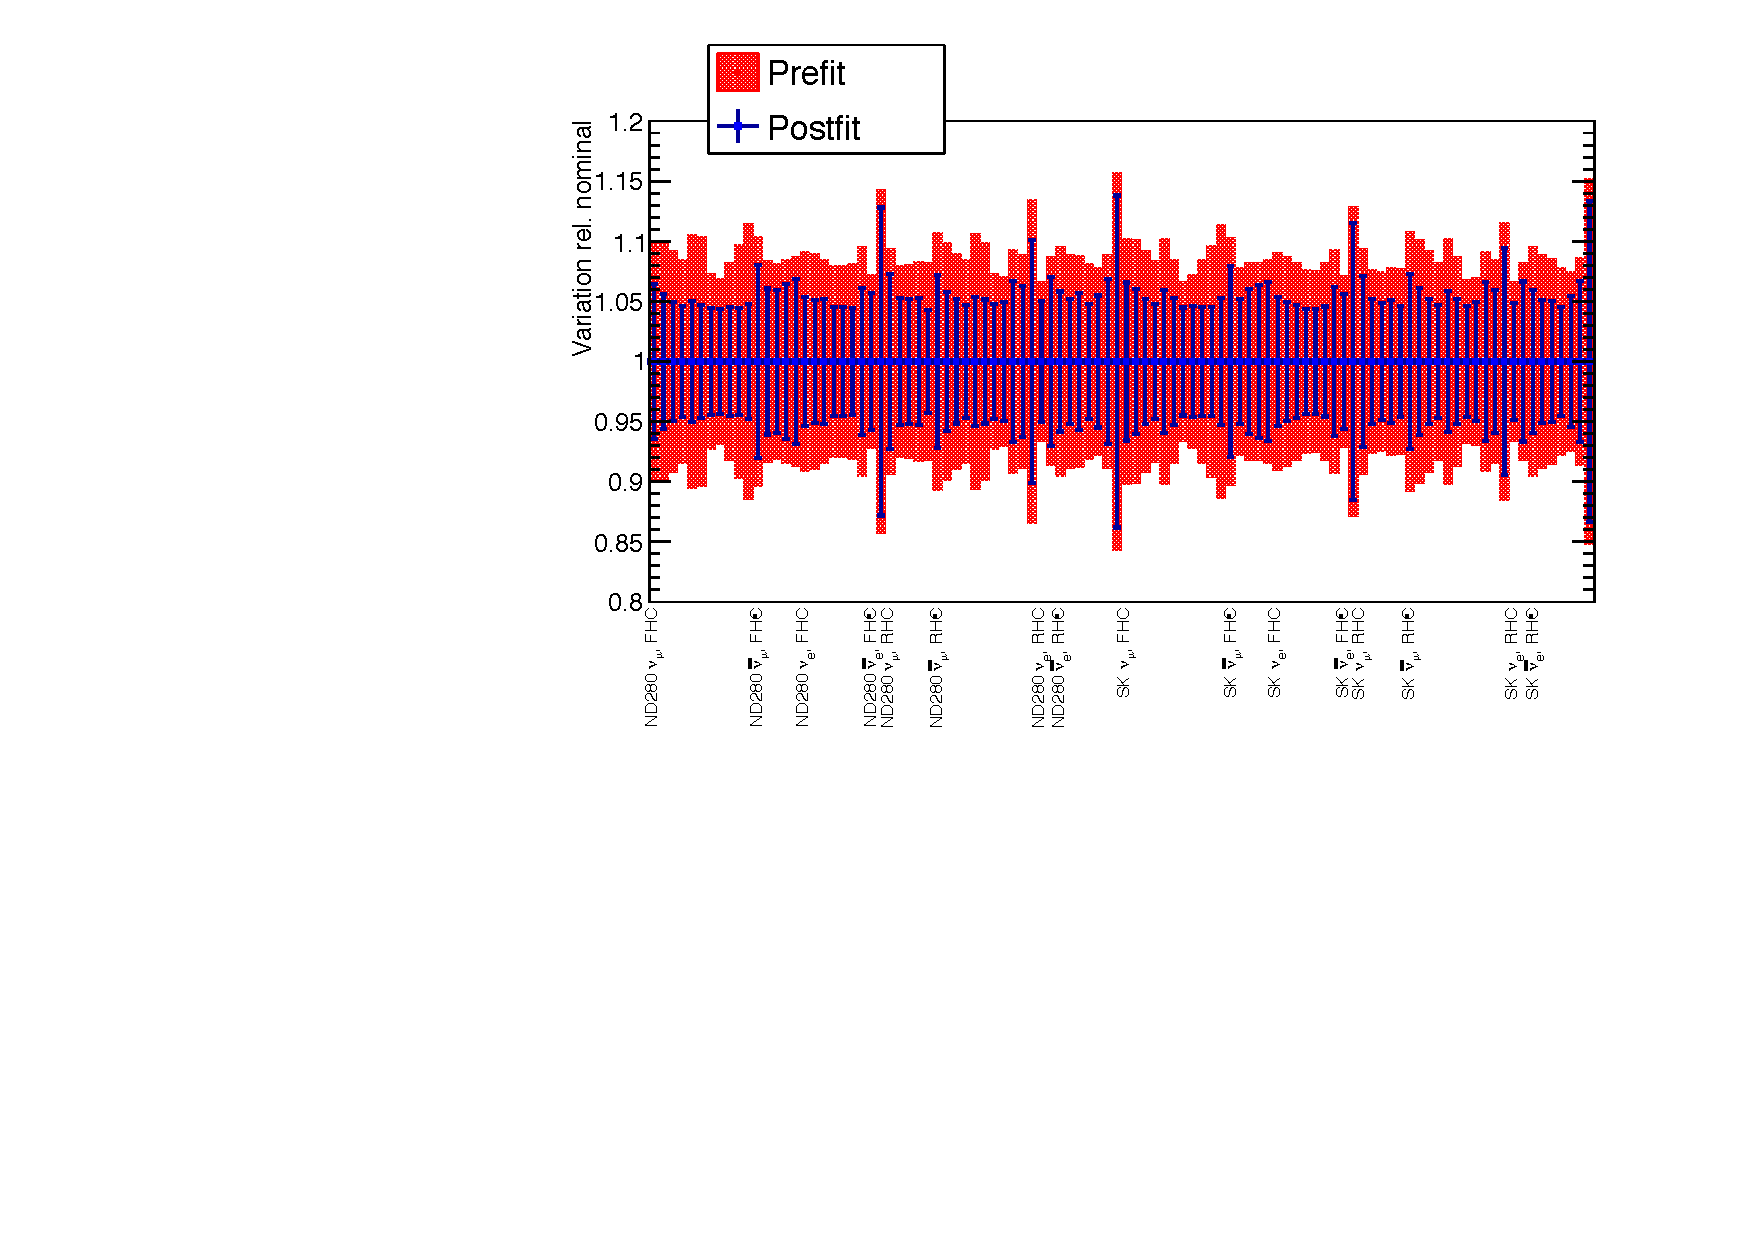
\includegraphics[width=\textwidth, trim={10mm 17mm 15mm 0mm}, clip, page=1]{figures/mach3/banff/asimov_banff_flux}
		\caption{Flux parameters}
	\end{subfigure}
	\begin{subfigure}[t]{0.49\textwidth}
		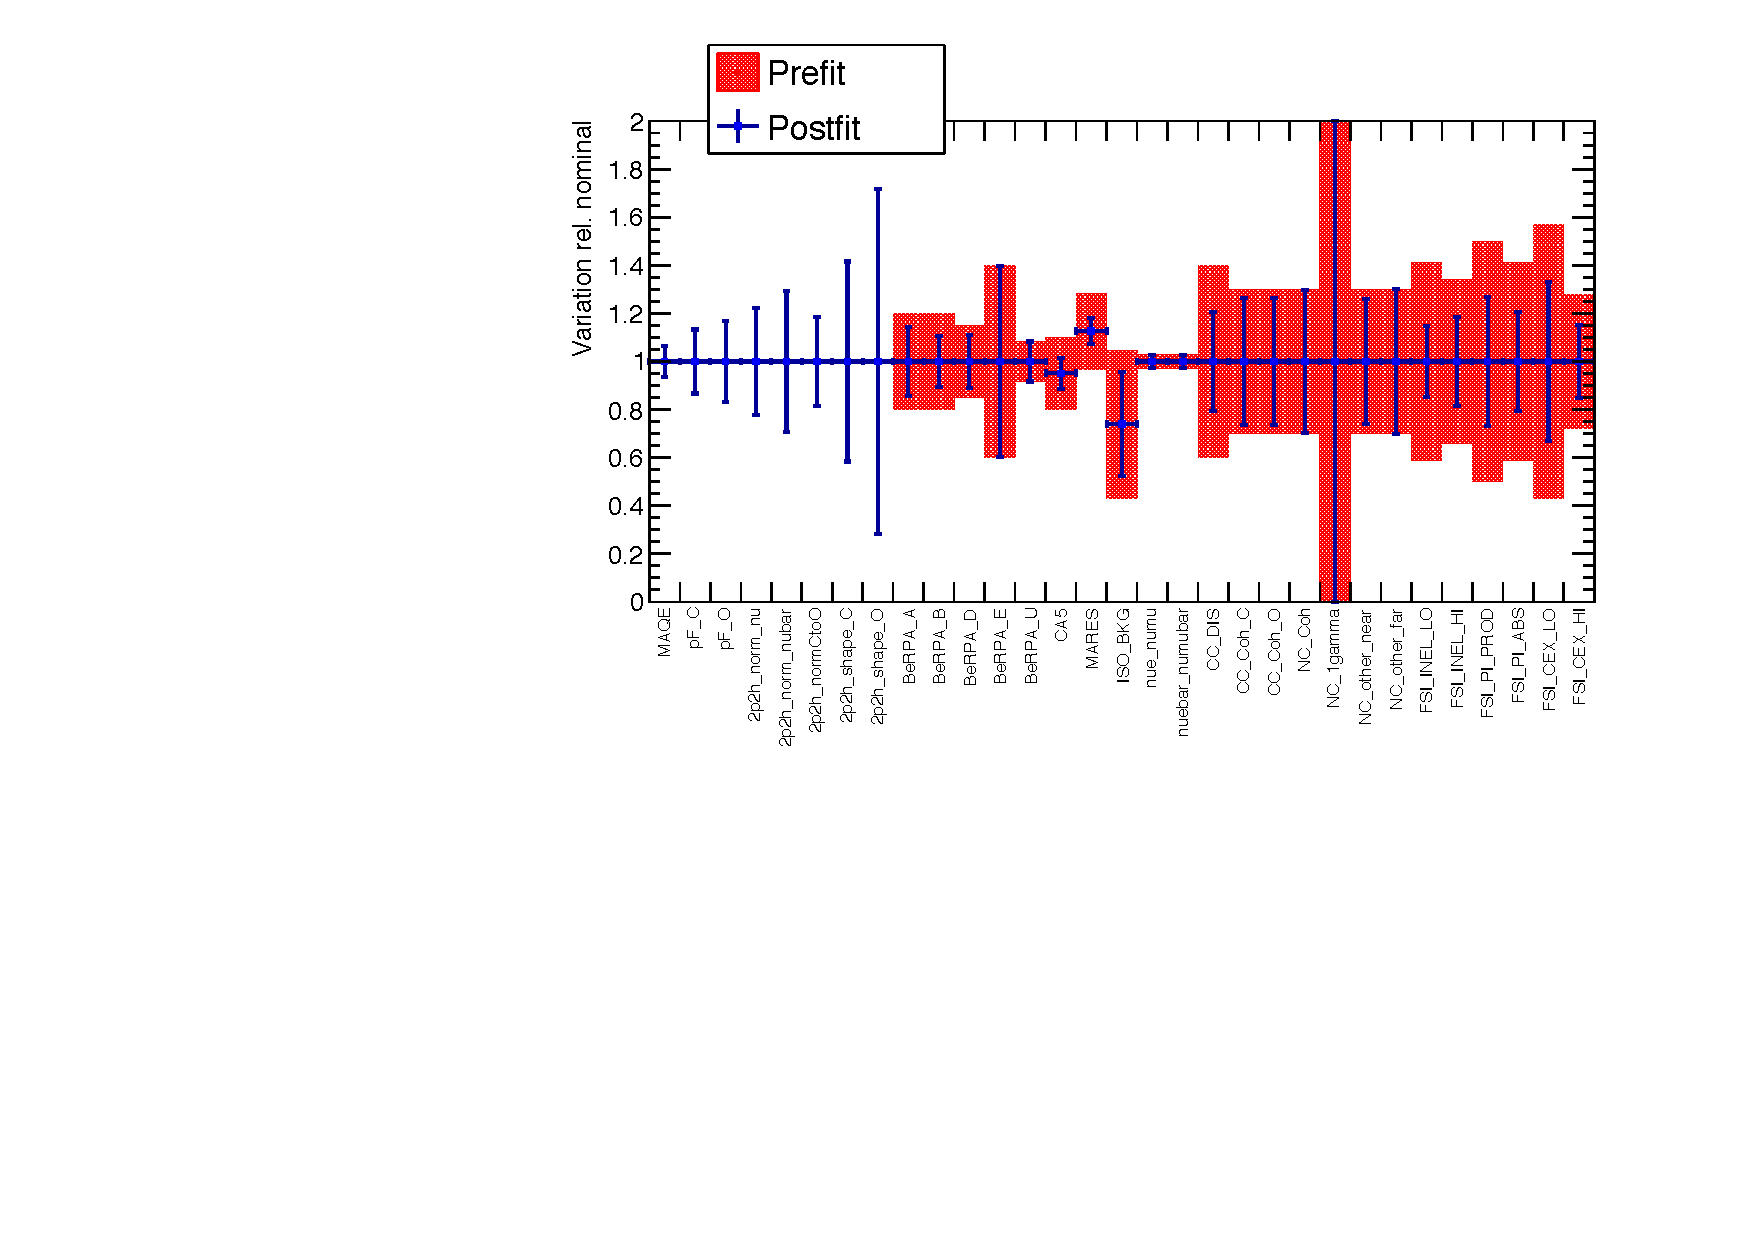
\includegraphics[width=\textwidth, trim={10mm 15mm 15mm 0mm}, clip, page=1]{figures/mach3/banff/asimov_banff_xsec}
		\caption{Interaction parameters}
	\end{subfigure}
	\caption{BANFF post-fit parameter when fitting the Asimov data set}
	\label{fig:banff_asimov}
\end{figure}

\section{Data fit}
We compare the global minimum from BANFF to the 1D marginalised posteriors from MaCh3, keeping the marginalisation issues detailed in \autoref{sec:marginalisation} in mind.

The flux parameters are compared in \autoref{fig:banff_mach3_flux} and we see a consistent shift in the parameters. The shapes are near identical, with BANFF seeing consistently higher flux parameters. This is largely expected due to the correlations of the flux with interaction parameters that showed marginalisation biases in the Asimov fit. The uncertainties on each of the parameters is consistent.
\begin{figure}[h]
	\begin{subfigure}[t]{0.49\textwidth}
		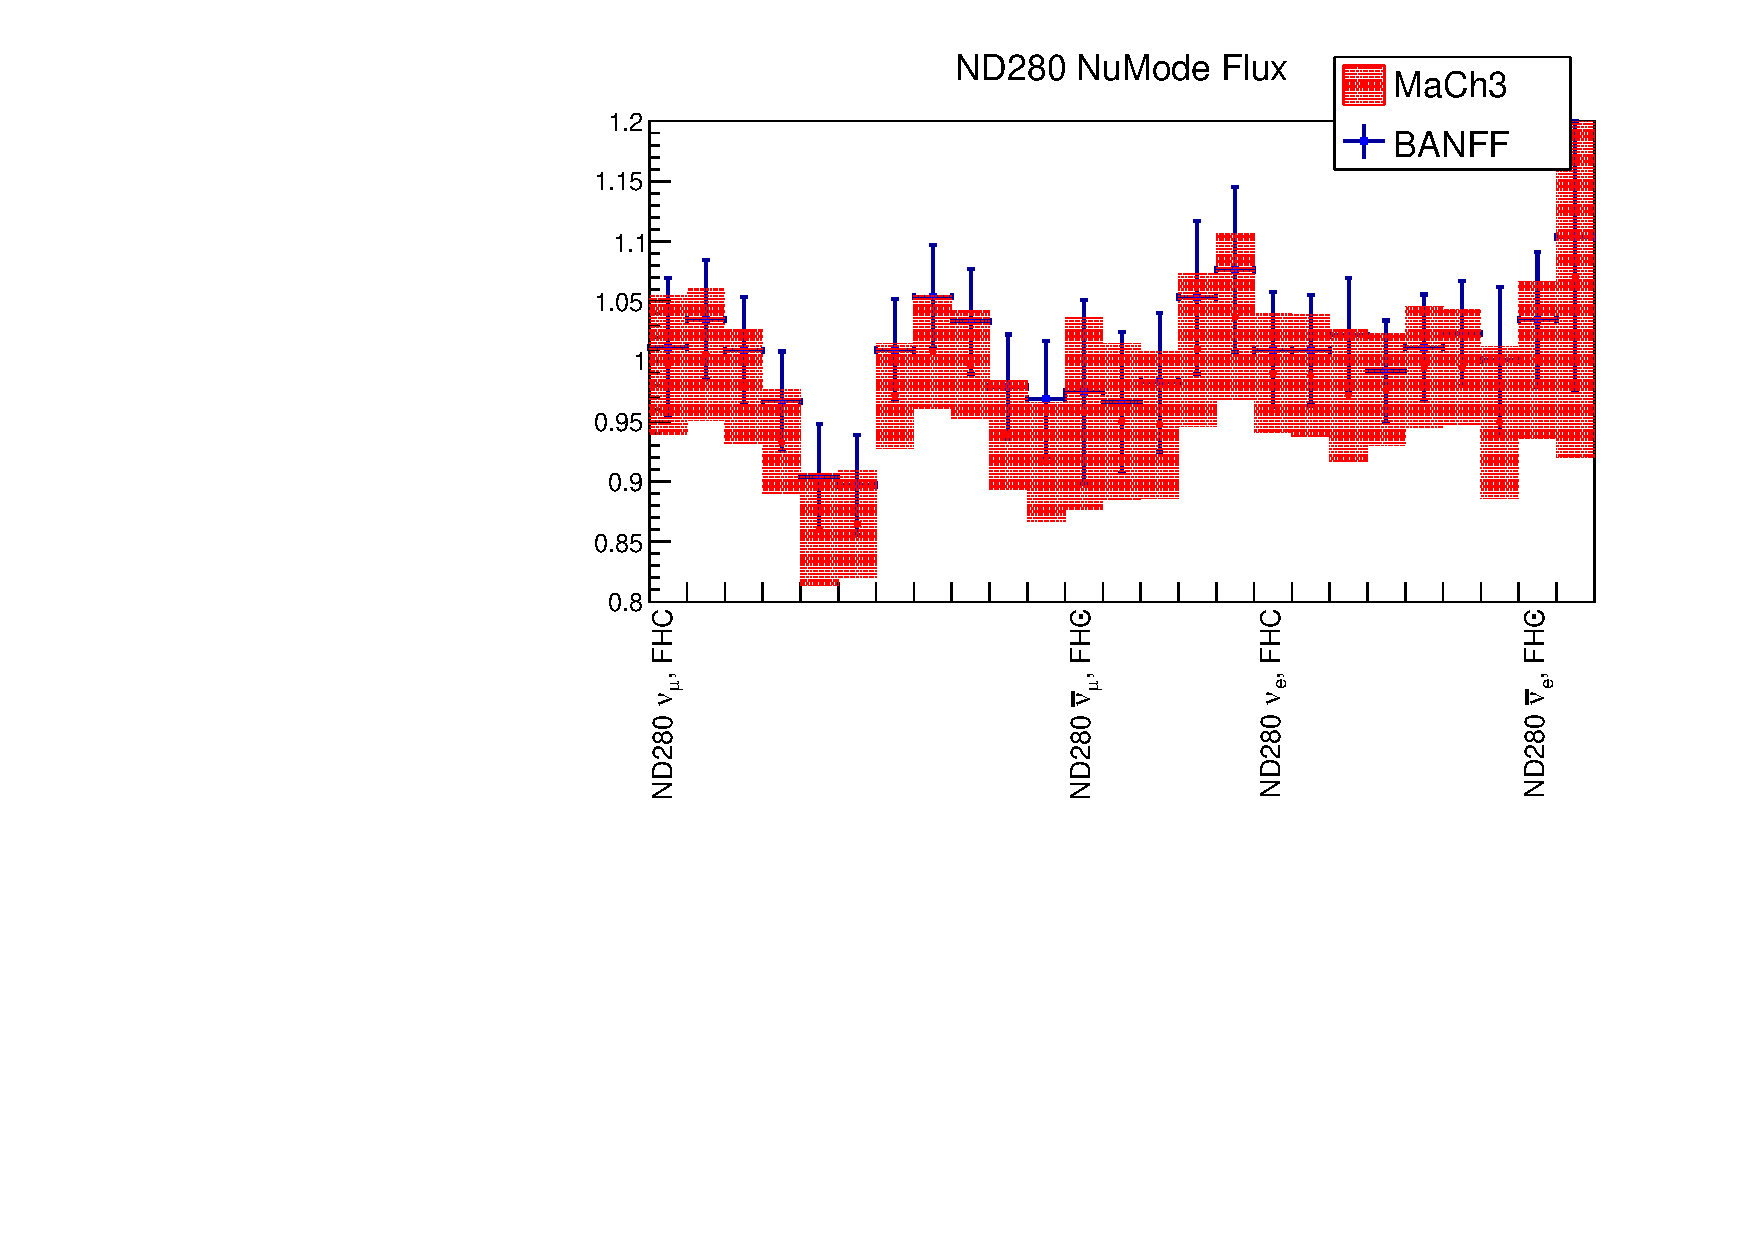
\includegraphics[width=\textwidth, trim={10mm 0mm 18mm 0mm}, clip, page=1]{figures/mach3/banff/mach3banff}
	\end{subfigure}
	\begin{subfigure}[t]{0.49\textwidth}
		\includegraphics[width=\textwidth, trim={10mm 0mm 18mm 0mm}, clip, page=2]{figures/mach3/banff/mach3banff}
	\end{subfigure}
	
	\begin{subfigure}[t]{0.49\textwidth}
		\includegraphics[width=\textwidth, trim={10mm 10mm 18mm 0mm}, clip, page=3]{figures/mach3/banff/mach3banff}
	\end{subfigure}
	\begin{subfigure}[t]{0.49\textwidth}
		\includegraphics[width=\textwidth, trim={10mm 10mm 18mm 0mm}, clip, page=4]{figures/mach3/banff/mach3banff}
	\end{subfigure}
	\caption{Flux parameters post-fit for BANFF and MaCh3}
	\label{fig:banff_mach3_flux}
\end{figure}

\autoref{fig:banff_mach3_xsec} shows the post-fit interaction parameters where differences aren't as pronounced. The uncertainties on $p_F$ are slightly different due to the method of evaluating the error (arithmetic mean) and the non-Gaussian shape of the one dimensional posterior. 2p2h normalisations and BeRPA A and B are different, as expected from the marginalisation bias present in the Asimov. The CC DIS parameter is also ``fit lower'' in MaCh3, likely due to the correlations with the flux parameters which are also fit higher.
\begin{figure}[h]
	\begin{subfigure}[t]{0.49\textwidth}
		\includegraphics[width=\textwidth, trim={10mm 0mm 18mm 0mm}, clip, page=6]{figures/mach3/banff/mach3banff}
	\end{subfigure}
	\begin{subfigure}[t]{0.49\textwidth}
		\includegraphics[width=\textwidth, trim={10mm 0mm 18mm 0mm}, clip, page=5]{figures/mach3/banff/mach3banff}
	\end{subfigure}
	\caption{Interaction parameters post-fit for BANFF and MaCh3}
	\label{fig:banff_mach3_xsec}
\end{figure}

Finally we can also compare the final event rates and test-statistics in \autoref{tab:banff_mach3_postfit_eventrate}. The difference in number of events is -15.38 (MaCh3 higher), corresponding to -0.02\%. The test-statistic from the samples differs by -11.96 and as expected BANFF is lower. Comparing to the total number of fit bins (1624) and degrees of freedom (938), the $\Delta\left(-2\ln\mathcal{L}_s/\text{nDOF}\right) \sim -0.01$. The sample with the largest difference in test-statistic are the 0$\pi$ selections and FGD2 CCOther, where the difference is approximately 2.
\begin{table}[h]
	\centering 
	\begin{tabular}{ l | c c | c c }
		\hline
		\hline
		Sample 		& \multicolumn{2}{c|}{Event rate} & \multicolumn{2}{c}{-$2\ln{\mathcal{L}}_{s}$} \\
		& BANFF         & MaCh3    & BANFF    & MaCh3 \\
		\hline
		FGD1 0$\pi$ 	& 17122.22 	& 17123.80 & 169.97   & 172.21 	\\ 
		FGD1 1$\pi$ 	& 4061.65 	& 4054.18  & 164.06   & 164.04 	\\ 
		FGD1 Other 	& 4095.58 	& 4103.96  & 223.49   & 224.03 	\\ 
		\hline
		FGD2 0$\pi$ 	& 17494.56 	& 17500.70 & 164.40   & 166.15 	\\ 
		FGD2 1$\pi$ 	& 3416.28 	& 3409.63  & 162.62   & 162.71 	\\ 
		FGD2 Other 	& 3915.36 	& 3914.40  & 168.82   & 171.17 	\\ 
		\hline
		FGD1 1Trk 	& 3503.79 	& 3509.37  & 117.79   & 117.80 	\\ 
		FGD1 NTrk 	& 1052.69 	& 1062.70  & 74.98    & 76.50 	\\ 
		FGD2 1Trk 	& 3685.46  	& 3678.66  & 129.09   & 129.84 	\\ 
		FGD2 NTrk 	& 1097.38	& 1108.52  & 78.95    & 80.34 	\\ 
		\hline
		FGD1 1Trk 	& 1353.44 	& 1347.50  & 66.99    & 66.51 	\\ 
		FGD1 NTrk 	& 1354.02 	& 1358.99  & 62.00    & 61.75 	\\ 
		FGD2 1Trk 	& 1330.49 	& 1323.30  & 62.79    & 64.34 	\\ 
		FGD2 NTrk 	& 1263.12 	& 1265.69  & 75.17    & 75.70 	\\ 
		\hline
		Total 		& 64746.02      & 64761.40 & 1721.12  & 1733.08 	\\ 
		\hline
		\hline
	\end{tabular}
	\caption{Comparison of the event rates for data post-fit MC and -$2\ln{\mathcal{L}}_{s}$ contributions broken by sample for MaCh3 and BANFF}
	\label{tab:banff_mach3_postfit_eventrate}
\end{table}

\section{Post fit distributions}
We now compare the post-fit \pmu distributions from BANFF and MaCh3. The BANFF post-fit uses the parameter set which finds the global minimum, and MaCh3 uses the posterior predictive spectrum. The error on the MaCh3 prediction is the total uncertainty.

\autoref{fig:mach3_banff_postfit_fgd1} shows the post-fit predictions for FGD1 and \autoref{fig:mach3_banff_postfit_fgd2} for FGD2. The 0$\pi$, 1$\pi$ and 1 track distributions are identical to within 1\%. The Other and NTrk distributions show the largest differences, just above 2\% for FGD1 CCOther.
\begin{figure}
	\begin{subfigure}[t]{0.10\textwidth}
		\includegraphics[width=\textwidth, trim={0mm 0mm 0mm 0mm}, clip, page=2]{figures/mach3/banff/postfit_comp}
	\end{subfigure}
	
	\begin{subfigure}[t]{0.32\textwidth}
		\includegraphics[width=\textwidth, trim={0mm 0mm 10mm 7mm}, clip, page=3]{figures/mach3/banff/postfit_comp}
		\caption{0$\pi$}
	\end{subfigure}
	\begin{subfigure}[t]{0.32\textwidth}
		\includegraphics[width=\textwidth, trim={0mm 0mm 10mm 7mm}, clip, page=6]{figures/mach3/banff/postfit_comp}
		\caption{1$\pi$}
	\end{subfigure}
	\begin{subfigure}[t]{0.32\textwidth}
		\includegraphics[width=\textwidth, trim={0mm 0mm 10mm 7mm}, clip, page=9]{figures/mach3/banff/postfit_comp}
		\caption{Other}
	\end{subfigure}
	
	\begin{subfigure}[t]{0.24\textwidth}
		\includegraphics[width=\textwidth, trim={0mm 0mm 10mm 7mm}, clip, page=21]{figures/mach3/banff/postfit_comp}
		\caption{1Trk}
	\end{subfigure}
	\begin{subfigure}[t]{0.24\textwidth}
		\includegraphics[width=\textwidth, trim={0mm 0mm 10mm 7mm}, clip, page=24]{figures/mach3/banff/postfit_comp}
		\caption{NTrk}
	\end{subfigure}
	\begin{subfigure}[t]{0.24\textwidth}
		\includegraphics[width=\textwidth, trim={0mm 0mm 10mm 7mm}, clip, page=33]{figures/mach3/banff/postfit_comp}
		\caption{\numu 1Trk}
	\end{subfigure}
	\begin{subfigure}[t]{0.24\textwidth}
		\includegraphics[width=\textwidth, trim={0mm 0mm 10mm 7mm}, clip, page=36]{figures/mach3/banff/postfit_comp}
		\caption{\numu NTrk}
	\end{subfigure}
	\caption{FGD1 selections in \pmu with data, prefit, BANFF postfit and MaCh3 postfit}
	\label{fig:mach3_banff_postfit_fgd1}
\end{figure}

\begin{figure}
	\begin{subfigure}[t]{0.32\textwidth}
		\includegraphics[width=\textwidth, trim={0mm 0mm 10mm 7mm}, clip, page=12]{figures/mach3/banff/postfit_comp}
		\caption{0$\pi$}
	\end{subfigure}
	\begin{subfigure}[t]{0.32\textwidth}
		\includegraphics[width=\textwidth, trim={0mm 0mm 10mm 7mm}, clip, page=15]{figures/mach3/banff/postfit_comp}
		\caption{1$\pi$}
	\end{subfigure}
	\begin{subfigure}[t]{0.32\textwidth}
		\includegraphics[width=\textwidth, trim={0mm 0mm 10mm 7mm}, clip, page=18]{figures/mach3/banff/postfit_comp}
		\caption{Other}
	\end{subfigure}
	
	\begin{subfigure}[t]{0.24\textwidth}
		\includegraphics[width=\textwidth, trim={0mm 0mm 10mm 7mm}, clip, page=27]{figures/mach3/banff/postfit_comp}
		\caption{1Trk}
	\end{subfigure}
	\begin{subfigure}[t]{0.24\textwidth}
		\includegraphics[width=\textwidth, trim={0mm 0mm 10mm 7mm}, clip, page=30]{figures/mach3/banff/postfit_comp}
		\caption{NTrk}
	\end{subfigure}
	\begin{subfigure}[t]{0.24\textwidth}
		\includegraphics[width=\textwidth, trim={0mm 0mm 10mm 7mm}, clip, page=39]{figures/mach3/banff/postfit_comp}
		\caption{\numu 1Trk}
	\end{subfigure}
	\begin{subfigure}[t]{0.24\textwidth}
		\includegraphics[width=\textwidth, trim={0mm 0mm 10mm 7mm}, clip, page=42]{figures/mach3/banff/postfit_comp}
		\caption{\numu NTrk}
	\end{subfigure}
	\caption{FGD2 selections in \pmu with data, prefit, BANFF postfit and MaCh3 postfit}
	\label{fig:mach3_banff_postfit_fgd2}
\end{figure}